%L'introduction est une section requise dans un rapport technique. Introduisez votre travail, l'idée de départ et les objectifs attendus. Un lecteur qui découvrirait votre projet au travers de cette introduction devrait ainsi être capable d'en comprendre le cadre, l'idée générale et les aboutissants du projet.
Dans le cadre des études à la HEIG-VD, un travail de Bachelor et demandé en fin d'études. Ce dernier représente un projet sur un semestre. 

\section{Contexte}
%Cette section \underline{n'est pas obligatoire}, mais elle est souvent présente dans un rapport technique pour compléter l'introduction et définir le contexte du travail \cad le cadre formel dans lequel le travail est mené.
Dans le domaine de la santé, les nouveau-nés sont des patients requérant des soins très spécifiques, et tout particulièrement en cas de 
naissance prématurée. Un monitoring précis de leurs paramètres vitaux est alors indispensable pour permettre au personnel médical d'effectuer 
les soins les plus adaptés. Parmi ces paramètres le monitoring de l'assistance respiratoire est doublement utile : d'une part, il permet le 
contrôle précis de cette assistance en cas de détresse respiratoire, et d'autre part la mesure du débit respiratoire couplé au taux d'oxygène 
et de dioxyde de carbone donne des informations précieuses sur l'énergie dépensé par ces petits organismes. Cependant, les très petits volumes 
pulmonaires ainsi que des fréquences respiratoires élevées pousse les appareils conventionnels à leurs limites de détection. Des appareils plus 
adaptés à ces contraintes doivent être développés, qui d'une part doivent drastiquement minimiser les volumes morts qui fausse l'estimation du 
volume pulmonaire, et d'autre part doivent avoir une réponse temporelle très rapide. 

Ce travail de Bachelor porte sur la faisabilité d'un débitmètre respiratoire par nanotechnologie, qui mesurerait le flux d'air entrant et 
sortant sans volume mort et avec un temps de réponse inférieure à 100 ms. 

Ce projet vise ainsi à fabriquer des débitmètres par nanotechnologie et de développer un banc de test ad hoc pour en mesurer les performances.  

\section{Objectifs}
Ce travail de Bachelor vise à démontrer la faisabilité de débitmètre respiratoire utilisant des capteurs élaborés par une nanotechnologie à 
faibles coûts. Il se décline en quatre objectifs pratiques : \\
\vspace{0.2cm}
\textbf{Objectif 1} - Élaboration d'un cahier de spécifications \& d'un catalogue de solutions. \\
\vspace{0.2cm}
\textbf{Objectif 2} - Conception et réalisation d'un débitmètre par nanotechnologie. \\
\vspace{0.2cm}
\textbf{Objectif 3} - Conception et réalisation d'un banc de test dédié au débitmètre.\\
\vspace{0.2cm}
\textbf{Objectif 4} - Qualification des performances du débitmètre.

\section{État de l'art}
\subsection{Débitmètres néonatals sur le marché}
Plusieurs entreprises proposent des débitmètres néonatals. Ces entreprises ont été regroupées dans le tableau ci-dessous avec les 
technologies de capteur utilisées. \\
\begin{table}[H]
    \centering
    \begin{tabular}{|c|c|}
        \hline
        \textbf{Entreprises} & \textbf{Technologie}                \\
        \hline
        Sensirion            & Capteur thermique de débit massique \\
        \hline
        Mim-Germany          & Anémomètre à fil chaud double       \\
        \hline
        Europlaz             & Anémomètre à fils chauds            \\
        \hline
        Draeger              & Anémomètre à fil chaud              \\
        \hline
    \end{tabular}
    \caption{Débitmètres pédiatriques sur le marché}
    \label{tab:debitmetreMarche}
\end{table}


\subsection{Revues scientifiques}
Les revues scientifiques sont également des ressources intéressantes à considérer pour l'élaboration de l'état de l'art. En effet, les 
articles scientifiques vont permettre d'établir une liste des techniques déjà exploitées, leur fonctionnement détaillé ainsi que leurs 
performances. \\
\begin{figure}[H]
    \hspace{-1cm}
    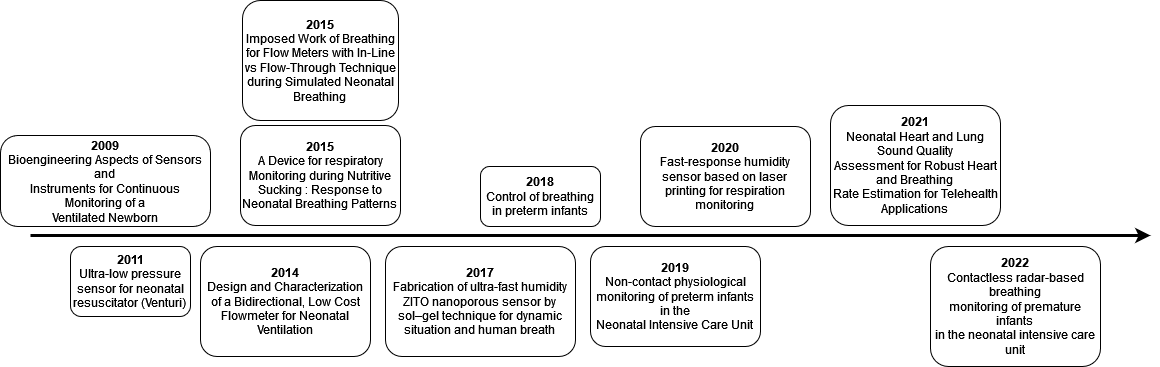
\includegraphics[scale = 0.45]{images/DRP_Etat_de_l_art.png}
    \caption{Articles scientifiques par ordre chronologique}
    \label{fig:articlesChrono}
\end{figure}

Les articles pertinents pour ce Travail de Bachelor sont résumés dans ce chapitre et classé par ordre chronologique sur la figure 
\ref{fig:articlesChrono}. \\

Les principales technologies exploitées comme débitmètre pédiatrique sont passée en revue ci-dessous. 

\subsubsection{Effet de Venturi}
Le débit respiratoire est mesuré grâce à une différence de pression. Cette différence de pression est engendré par un rétrécissement de 
l'espace de circulation du gaz (principe de Venturi) \cite{oberg_biomedical_2011}. 
\begin{figure}[H]
    \centering
    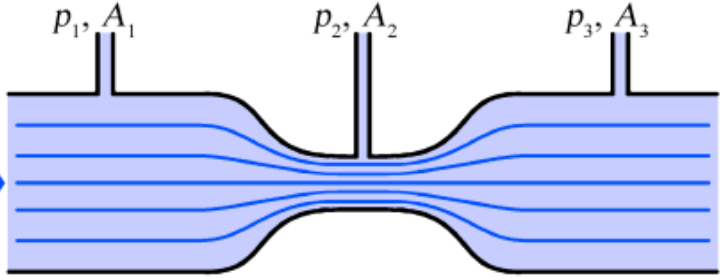
\includegraphics[scale = 0.5]{assets/figures/Venturi.png}
    \caption{Effet de Venturi \cite{oberg_biomedical_2011}}
    \label{fig:venturi}
\end{figure}

La figure \ref{fig:venturi} illustre l'effet Venturi. Avec un rétrécissement de la partie centrale d'un tube, le fluide traversant le dispositif 
sera accéléré et subira également une dépression à cet endroit. Ainsi, en mesurant la pression à différents endroits du tube, il est possible 
de calculer le flux d'air. \\

C'est la technologie utilisée par les pneumotachographes (le pneumotachographe de Fleisch par exemple). Mais elle peut également être utilisée 
dans une application quelque peu différente. En effet, un article mentionne son utilisation dans un ressuscitateur \cite{jacq_ultra-low_2011}. 
Un tel appareil permet la réanimation du patient qui ne respire plus. Le ressuscitateur gonfle les poumons d'air et ainsi s'assure qu'un bon 
taux d'oxygène circule dans le patient. \\
Pour les nouveaux-né, la quantité d'air injectée dans les poumons doit être mesurée, car un trop grand débit pourrait rapidement engendrer 
des dégâts. \\
Couplé au système de Venturi, un capteur de force vient mesurer la pression et le volume d'air passant par le ressuscitateur. \\

Cette technologie a l'avantage d'être connue et utilisée depuis maintenant longtemps. Elle offre alors une certaine confiance aux utilisateurs. 
De plus, elle procure un débit linéaire. \\
Cependant, elle possède le désavantage d'être sensible aux conditions environnementales. Un thermostat est donc souvent nécessaire \cite{fischberg_pratique_2009}.

\subsubsection{Anémomètre à fils chauds}
Par la suite, il est expliqué que le pneumotachographe est gentiment remplacé par les anémomètres à fil chaud. Ces capteurs sont 
constitués d'un ou plusieurs fils chauffés par une source de courant. Lorsqu'un flux d'air va souffler sur le fil, ce dernier va être refroidi. 
Le niveau de refroidissement est directement lié au débit du flux \cite{oberg_biomedical_2011}. \\
L'article susmentionné conseil l'utilisation des anémomètres à deux fils contrairement à ceux à un seul fil qui aurait des performances 
moindres. 
L'anémomètre à fils chauds est une technologie incorporée par exemple dans la machine "Draeger Babylog", marque mentionnée dans le tableau \ref{tab:debitmetreMarche}. \\

L'avantage de cette technologie est qu'elle possède une faible résistance intrinsèque et est moins sensible à l'environnement. Toutefois, les 
filaments sont plus fragiles et deux filaments sont nécessaires pour des questions de fiabilité du résultat. 

\subsubsection{Transfert de chaleur entre deux transistors}

Une autre technologie pour débitmètre consiste à utiliser le transfert de chaleur entre deux transistors. 
\begin{figure}[H]
    \centering
    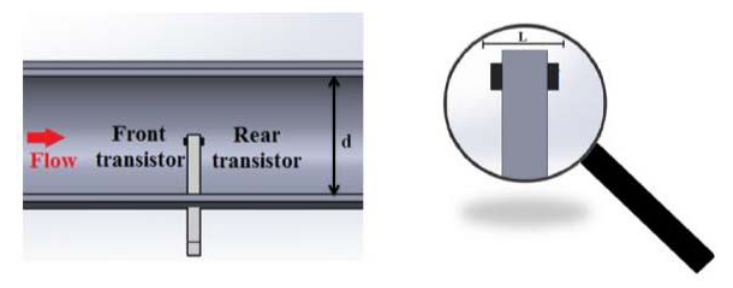
\includegraphics[scale = 0.5]{images/Debitmetre_transistors.png}
    \caption{Principe du débitmètre à transistors\cite{giorgino_design_2014}}
    \label{fig:transistors}
\end{figure}

C'est un principe encore innovant décrit dans l'article \cite{giorgino_design_2014}, utilisé dans l'article \cite{rosi_device_2016} et illustré 
par la figure \ref{fig:transistors}. 
Le premier transistor (appelé Front transistor) est placé perpendiculairement au flux d'air sur un PCB. \\
Le second (Rear transistor) est fixé de l'autre côté du PCB, dos à dos avec le premier transistor (cf. figure \ref{fig:transistors}) et mesure la 
chaleur émise par le Front transistor et transférée par le flux d'air. \\
De cette manière, le capteur sera capable de distinguer une expiration d'une inspiration. Le temps de réponse d'un tel capteur serait 
d'environ 340 ms. C'est un très bon temps de réponse en comparaison des capteurs médicaux existants sur le marché. Cependant, diverses améliorations 
doivent encore être faites avant de pouvoir utiliser une telle technologie. 

\begin{comment}
L'article suivant est intéressant au niveau du listage des débitmètres pédiatriques existants \cite{}. En effet, il étudie les différents fonctionnements 
existants et compare les signaux obtenus. Étant donné que cet article étudie plus précisément une caractéristique ("IN-line" vs "Flow-Through"), 
il est moins important dans le cadre de ce projet.\\
\end{comment}

\subsubsection{Caméra}
La thématique de l'article \cite{villarroel_non-contact_2019} repose sur une technologie de monitoring non invasive. Elle utilise une caméra qui suit les mouvements du nouveaux-né. 
Cette technologie permet également d'enregistrer d'autres signaux tels que la fréquence cardiaque, mais elle requiert encore quelques améliorations 
ainsi que quelques recherches supplémentaires. \\

Cette technologie a le grand avantage d'être non invasive, mais n'est pas encore aboutie. 

\subsubsection{Mesure thermique par l'entreprise Sensirion}
L'entreprise Sensirion propose une technologie basée sur des mesures de températures. Une membrane incorporée dans une puce est utilisé comme 
capteur de débit. Un flux d'air vient transférer la chaleur du corps de chauffe placé au milieu de la membrane. Deux capteurs de température 
sont placés en aval et en amont du corps de chauffe, en direction du flux. Un signal précis engendré par la différence de température en aval et  
en amont sera finalement mesurable. 
\begin{figure}[H]
    \centering
    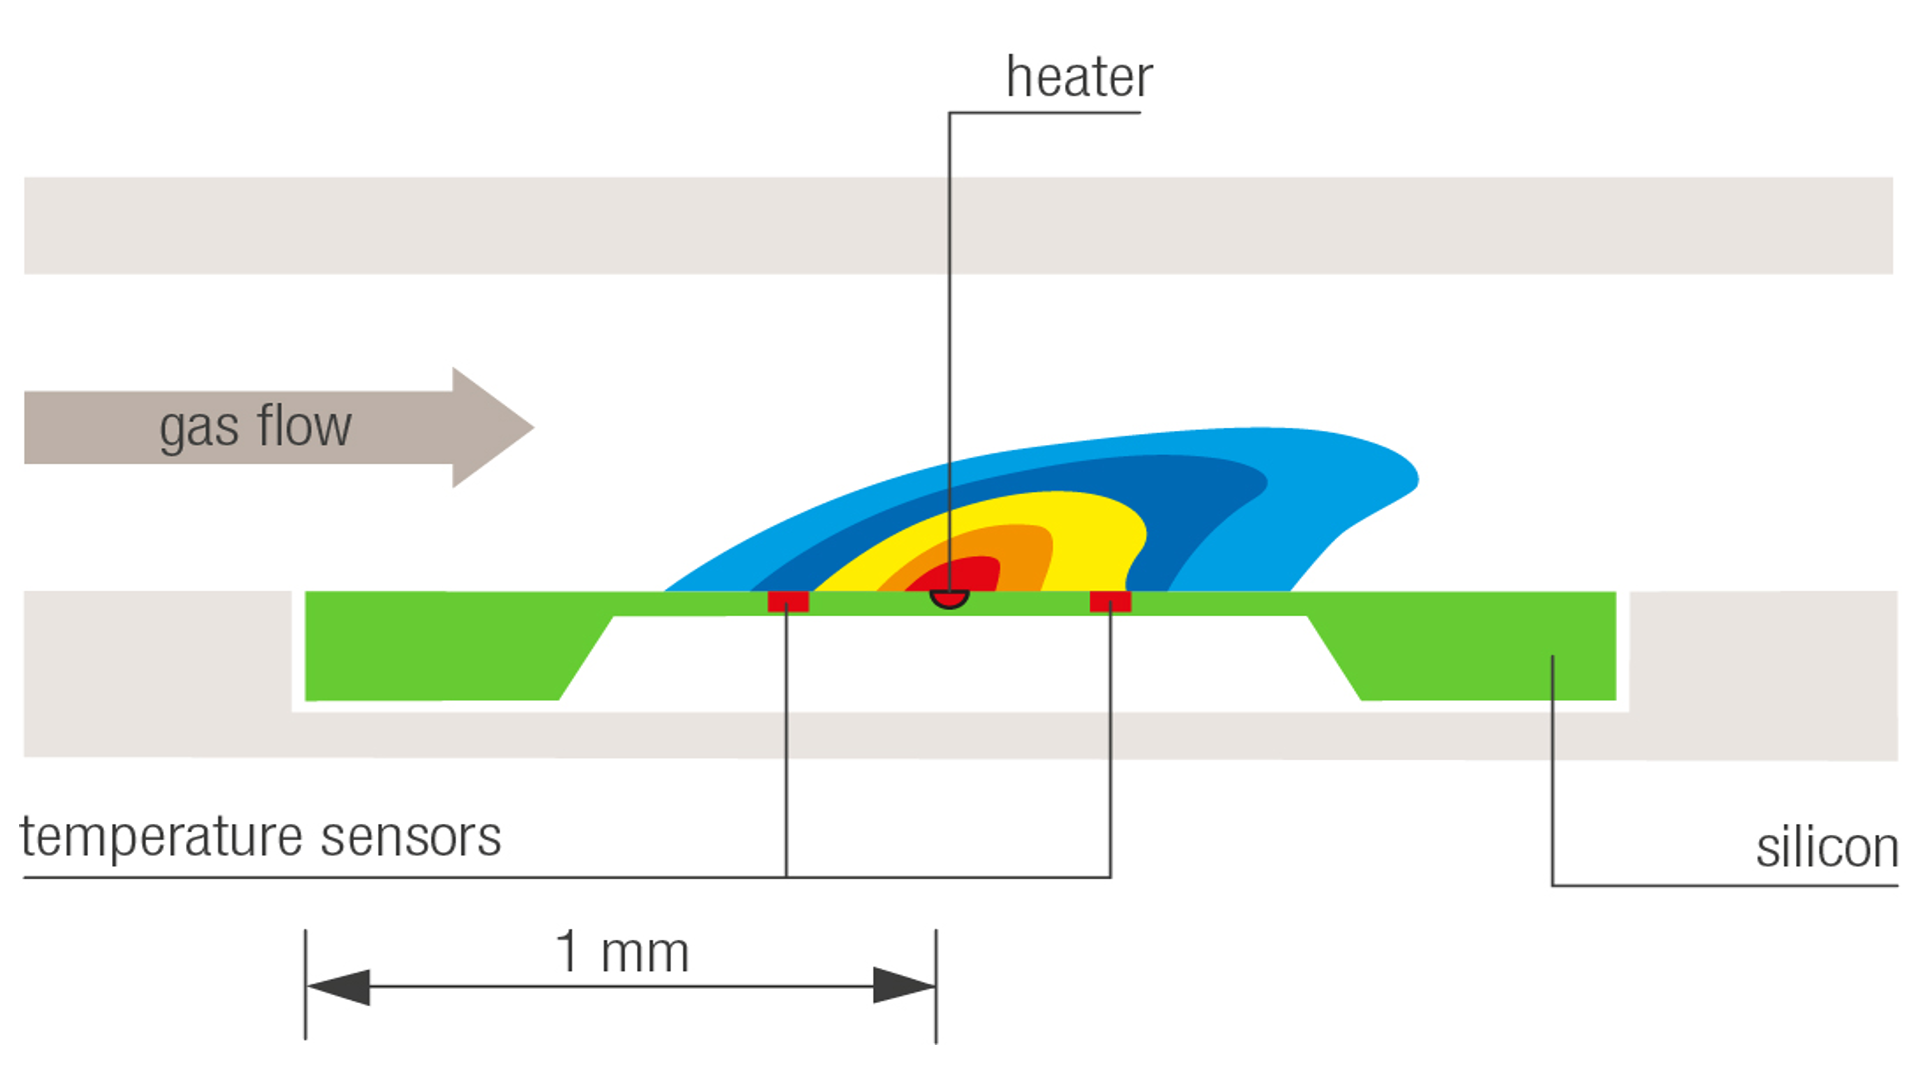
\includegraphics[scale = 0.15]{assets/figures/Sensirion_tech.png}
    \caption{Technologie proposée par Sensirion\cite{noauthor_smart_nodate}}
    \label{fig:sensirion}
\end{figure}

\subsubsection{Nanotechnologie}
Un autre article mentionne les membranes nanoporeuses comme capteur \cite{moharamzadeh_fabrication_2018}. Bien que cette technique se rapproche 
de notre application, ces capteurs sont pour l'humidité et non le débit respiratoire. Des nanostructures d'oxyde de Zinc sont utilisées, car 
elles possèdent de bonnes propriétés physiques et chimiques. Étant donné que l'humidité et le débit respiratoire sont en lien, l'article évoque 
également le débit, cependant, il ne l'étudie pas plus en détail. \\
Toutefois, un temps de réponse plutôt bon, de l'ordre de la seconde est attendu avec une telle technologie. 

\section{Benchmarking}
Avec les différentes informations récoltées de l'état de l'art, un benchmarking peut être élaboré. Ce dernier est composé de différentes valeurs 
de performance à atteindre dans l'idéal. 

\begin{table}[H]
    \centering
    \begin{tabular}{|c|c|}
        \hline
        \textbf{Plage de débit}           & $\pm 8$ l/min     \\
        \hline
        \textbf{Sensibilité de détection} & < 0.1 l/min       \\
        \hline
        \textbf{Temps de réponse}         & < 340 ms          \\
        \hline
        \textbf{Fréquence de respiration} & entre 0.3 et 3 Hz \\
        \hline
        \textbf{Diamètre des conduits}    & < 10 mm           \\
        \hline
    \end{tabular}
    \caption{Benchmarking}
    \label{fig:benchmarking}
\end{table}


\section{Fonctionnement du débitmètre respiratoire pédiatrique}
Ce travail de Bachelor est donc une recherche à propos d'un débitmètre dont le principe de fonctionnement est encore innovant. \\

Le capteur développé repose sur le phénomène de l'effet Seebeck, phénomène que l'on peut également retrouver dans les thermocouples. L'effet 
Seebeck est le suivant :\\

Lorsqu'un matériau conducteur ou semiconducteur est soumis à un gradient de température, les électrons libres vont se déplacer du chaud vers le 
froid : une tension s'établit alors entre les extrémités du matériau (Figure \ref{fig:Seebeck}\cite{instrumentys_effet_2021}).
\begin{figure}[H]
    \centering
    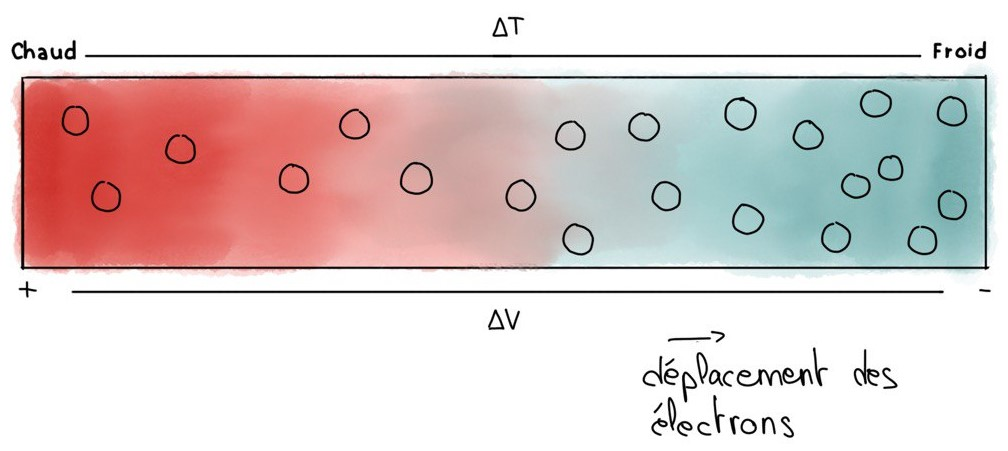
\includegraphics[scale = 0.3]{images/Seebeck.jpg}
    \caption{Effet de Seebeck}
    \label{fig:Seebeck}
\end{figure}

La tension est calculée grâce à la formule suivante :
\[V = S \cdot (T_{chaude} - T_{froide})\]
Avec S, le coefficient Seebeck de l'ordre de quelques $\upmu$V/K\\

Le principe du débitmètre nanostructuré est illustré sur la figure \ref{fig:schema_coupe} : un corps de chauffe est encadré par deux vias de nanofils 
thermoélectriques formants chacun un thermocouple. Un flux d'air déportera la chaleur de façon à refroidir un thermocouple et réchauffer l'autre. La 
différence de température indiquée par la tension Seebeck permettra de déduire le débit du flux d'air. De la très faible inertie thermique des 
structures nanofils est attendue une réponse temporelle très rapide. 
\begin{figure}[H]
    \centering
    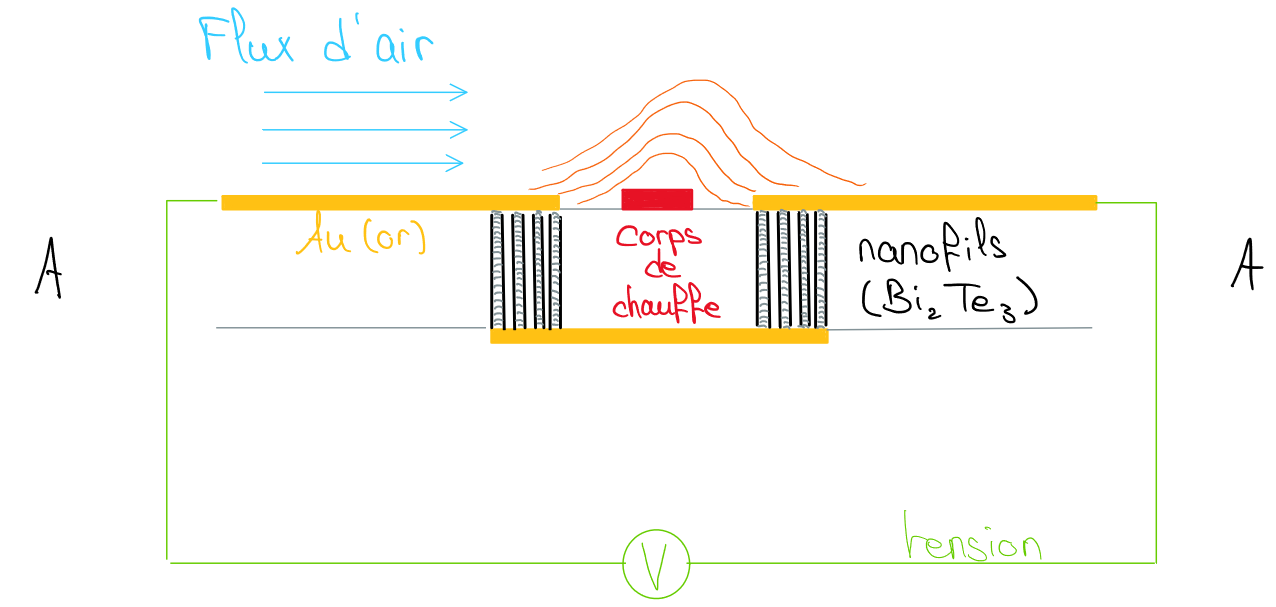
\includegraphics[scale = 0.4]{images/CapteurFUN.png}
    \caption{Schéma de principe du débitmètre nanostructuré}
    \label{fig:schema_coupe}
\end{figure}

\section{Livrables}
\begin{itemize}
    \item Cahier de spécifications
    \item Débitmètre fonctionnel
    \item Banc de test
    \item Rapport technique
\end{itemize}

\newpage
\section{Planification}
\begin{table}[H]
    \centering
    \begin{tabular}{lllllllll}
                                                                                                                  &                                                                               &                                                                               &                                                                               &                                                                               &                                                                               &                       &  & \\ \cline{2-9}
        \multicolumn{1}{l|}{}                                                                                     & \multicolumn{1}{c|}{\begin{tabular}[c]{@{}c@{}}23.02 - \\ 23.03\end{tabular}} & \multicolumn{3}{c|}{\begin{tabular}[c]{@{}c@{}}23.03 - \\ 09.05\end{tabular}} & \multicolumn{1}{c|}{\begin{tabular}[c]{@{}c@{}}09.05 - \\ 08.06\end{tabular}} & \multicolumn{2}{c|}{\begin{tabular}[c]{@{}c@{}}15.06 - \\ 13.07\end{tabular}} & \multicolumn{1}{c|}{\begin{tabular}[c]{@{}c@{}}13.07 - \\ 27.07\end{tabular}}                              \\ \hline
        \multicolumn{1}{|l|}{\begin{tabular}[c]{@{}l@{}}Prise en main du projet \\ et état de l'art\end{tabular}} & \multicolumn{1}{l|}{\cellcolor[HTML]{9AFF99}}                                 & \multicolumn{3}{l|}{}                                                         & \multicolumn{1}{l|}{}                                                         & \multicolumn{2}{l|}{}                                                         & \multicolumn{1}{l|}{}                                                                                      \\ \hline
        \multicolumn{1}{|l|}{\begin{tabular}[c]{@{}l@{}}Formation à l'électro-\\ déposition\end{tabular}}         & \multicolumn{1}{l|}{}                                                         & \multicolumn{2}{l|}{\cellcolor[HTML]{9AFF99}}                                 & \multicolumn{1}{l|}{}                                                         & \multicolumn{1}{l|}{}                                                         & \multicolumn{2}{l|}{}                                                         & \multicolumn{1}{l|}{}      \\ \hline
        \multicolumn{1}{|l|}{\begin{tabular}[c]{@{}l@{}}Conception du support du \\ capteur\end{tabular}}         & \multicolumn{1}{l|}{}                                                         & \multicolumn{1}{l|}{}                                                         & \multicolumn{3}{l|}{\cellcolor[HTML]{9AFF99}}                                 & \multicolumn{2}{l|}{}                                                         & \multicolumn{1}{l|}{}                                                                                      \\ \hline
        \multicolumn{1}{|l|}{Rendu intermédiaire}                                                                 & \multicolumn{1}{l|}{}                                                         & \multicolumn{3}{l|}{}                                                         & \multicolumn{1}{l|}{}                                                         & \multicolumn{1}{l|}{\cellcolor[HTML]{9AFF99}}                                 & \multicolumn{1}{l|}{}                                                         & \multicolumn{1}{l|}{}      \\ \hline
        \multicolumn{1}{|l|}{Conception du banc de test}                                                          & \multicolumn{1}{l|}{}                                                         & \multicolumn{3}{l|}{}                                                         & \multicolumn{1}{l|}{}                                                         & \multicolumn{2}{l|}{\cellcolor[HTML]{9AFF99}}                                 & \multicolumn{1}{l|}{}                                                                                      \\ \hline
        \multicolumn{1}{|l|}{Mesures}                                                                             & \multicolumn{1}{l|}{}                                                         & \multicolumn{3}{l|}{}                                                         & \multicolumn{1}{l|}{}                                                         & \multicolumn{1}{l|}{}                                                         & \multicolumn{2}{l|}{\cellcolor[HTML]{9AFF99}}                                                              \\ \hline
        \multicolumn{1}{|l|}{Rapport}                                                                             & \multicolumn{8}{l|}{\cellcolor[HTML]{D3FDD3}}                                                                                                                                                                                                                                                                                                                                                                                              \\ \hline
    \end{tabular}
\end{table}

L'avancée du travail a été suivie par une séance hebdomadaire. 

\section{Plan du rapport}
La présentation du travail effectué est structurée en cinq chapitres distincts :
\begin{description}
    \item[Chapitre 1 -] Cahier des spécifications\\
        Revue de la littérature, rédaction d'un état de l'art et définition du benchmarking. \\
    \item[Chapitre 2 -] Conception et réalisation du capteur nanostructuré\\
        Électrodéposition, déposition physique en phase vapeur (\gls{pvd}), conditionnement du capteur (réalisation des supports)\\
    \item[Chapitre 3 -] Conception et réalisation du banc de test\\
        Commandes, études des différents composants du banc de test, réalisation, montage et validation\\
    \item[Chapitre 4 -] Qualification du capteur\\
        Définition d'un protocole de mesures, résultats et analyses\\
    \item[Chapitre 5 -] Conclusion\\
\end{description}

